% Options for packages loaded elsewhere
\PassOptionsToPackage{unicode}{hyperref}
\PassOptionsToPackage{hyphens}{url}
%
\documentclass[
  12pt,
]{article}
\usepackage{lmodern}
\usepackage{setspace}
\usepackage{amssymb,amsmath}
\usepackage{ifxetex,ifluatex}
\ifnum 0\ifxetex 1\fi\ifluatex 1\fi=0 % if pdftex
  \usepackage[T1]{fontenc}
  \usepackage[utf8]{inputenc}
  \usepackage{textcomp} % provide euro and other symbols
\else % if luatex or xetex
  \usepackage{unicode-math}
  \defaultfontfeatures{Scale=MatchLowercase}
  \defaultfontfeatures[\rmfamily]{Ligatures=TeX,Scale=1}
\fi
% Use upquote if available, for straight quotes in verbatim environments
\IfFileExists{upquote.sty}{\usepackage{upquote}}{}
\IfFileExists{microtype.sty}{% use microtype if available
  \usepackage[]{microtype}
  \UseMicrotypeSet[protrusion]{basicmath} % disable protrusion for tt fonts
}{}
\makeatletter
\@ifundefined{KOMAClassName}{% if non-KOMA class
  \IfFileExists{parskip.sty}{%
    \usepackage{parskip}
  }{% else
    \setlength{\parindent}{0pt}
    \setlength{\parskip}{6pt plus 2pt minus 1pt}}
}{% if KOMA class
  \KOMAoptions{parskip=half}}
\makeatother
\usepackage{xcolor}
\IfFileExists{xurl.sty}{\usepackage{xurl}}{} % add URL line breaks if available
\IfFileExists{bookmark.sty}{\usepackage{bookmark}}{\usepackage{hyperref}}
\hypersetup{
  pdftitle={Your Awesome Title},
  pdfauthor={Author One1* and Author Two2},
  hidelinks,
  pdfcreator={LaTeX via pandoc}}
\urlstyle{same} % disable monospaced font for URLs
\usepackage[margin=1in]{geometry}
\usepackage{longtable,booktabs}
% Correct order of tables after \paragraph or \subparagraph
\usepackage{etoolbox}
\makeatletter
\patchcmd\longtable{\par}{\if@noskipsec\mbox{}\fi\par}{}{}
\makeatother
% Allow footnotes in longtable head/foot
\IfFileExists{footnotehyper.sty}{\usepackage{footnotehyper}}{\usepackage{footnote}}
\makesavenoteenv{longtable}
\usepackage{graphicx}
\makeatletter
\def\maxwidth{\ifdim\Gin@nat@width>\linewidth\linewidth\else\Gin@nat@width\fi}
\def\maxheight{\ifdim\Gin@nat@height>\textheight\textheight\else\Gin@nat@height\fi}
\makeatother
% Scale images if necessary, so that they will not overflow the page
% margins by default, and it is still possible to overwrite the defaults
% using explicit options in \includegraphics[width, height, ...]{}
\setkeys{Gin}{width=\maxwidth,height=\maxheight,keepaspectratio}
% Set default figure placement to htbp
\makeatletter
\def\fps@figure{htbp}
\makeatother
% Make links footnotes instead of hotlinks:
\DeclareRobustCommand{\href}[2]{#2\footnote{\url{#1}}}
\setlength{\emergencystretch}{3em} % prevent overfull lines
\providecommand{\tightlist}{%
  \setlength{\itemsep}{0pt}\setlength{\parskip}{0pt}}
\setcounter{secnumdepth}{-\maxdimen} % remove section numbering
\usepackage{geometry}
\geometry{verbose,letterpaper,margin=2.45cm}

% \usepackage[breaklinks=true,pdfstartview=FitH,citecolor=blue]{hyperref}
\hypersetup{colorlinks,%
	citecolor=blue,%
	filecolor=red,%
	linkcolor=blue,%
	urlcolor=red,%
	pdfstartview=FitH}

% \usepackage[T1]{fontenc}
% \usepackage[utf8]{inputenc}
% \usepackage{textgreek}
\usepackage{babel}
% % \usepackage{microtype}
% % \usepackage{amsmath}
\usepackage[osf]{libertine}
\usepackage{libertinust1math}
\usepackage{inconsolata}

\usepackage{longtable}

\usepackage{booktabs}

\usepackage{setspace}
% \doublespacing

% \setstretch{1.8999999999999999}

\usepackage{lineno}
% \linenumbers

\usepackage{flafter}
\usepackage{float}

% \renewcommand{\rmdefault}{cmr}

\usepackage[document]{ragged2e}

% % flush left while keep identation
% \makeatletter
% \newcommand\iraggedright{%
%   \let\\\@centercr\@rightskip\@flushglue \rightskip\@rightskip
%   \leftskip\z@skip}
% \makeatother
% \raggedright

% make pdf as default figure format
\DeclareGraphicsExtensions{.pdf,.png, %
    .jpg,.mps,.jpeg,.jbig2,.jb2,.JPG,.JPEG,.JBIG2,.JB2}
    
% \DeclareUnicodeCharacter{3B1}{\ensuremath{\alpha}}
% \DeclareUnicodeCharacter{3B2}{\ensuremath{\beta}}
% \DeclareUnicodeCharacter{0394}{$\Delta$}

\usepackage[labelsep=period]{caption}
\captionsetup{labelfont=bf}
% \usepackage{caption}
% \DeclareCaptionLabelSeparator{vline}{ \textbf{|} }
% \captionsetup{labelsep=vline, labelfont = {bf}}
\usepackage{booktabs}
\usepackage{longtable}
\usepackage{array}
\usepackage{multirow}
\usepackage{wrapfig}
\usepackage{float}
\usepackage{colortbl}
\usepackage{pdflscape}
\usepackage{tabu}
\usepackage{threeparttable}
\usepackage{threeparttablex}
\usepackage[normalem]{ulem}
\usepackage{makecell}
\usepackage{xcolor}
\newlength{\cslhangindent}
\setlength{\cslhangindent}{1.5em}
\newenvironment{cslreferences}%
  {\setlength{\parindent}{0pt}%
  \everypar{\setlength{\hangindent}{\cslhangindent}}\ignorespaces}%
  {\par}

\title{Your Awesome Title}
\author{Author One\textsuperscript{1}* and Author Two\textsuperscript{2}}
\date{2021-11-02 15:56:55}

\begin{document}
\maketitle

% align only at left, not at right.
\renewcommand{\figurename}{{\textbf{Figure}}}
\renewcommand{\tablename}{{\textbf{Table}}}
% \iraggedright

\setstretch{1.5}
\footnotesize

\textsuperscript{1}Department of Biological Sciences, Louisiana State University, Baton Rouge, LA, USA\\
\textsuperscript{2}Center for Computation \& Technology, Louisiana State University, Baton Rouge, LA, USA

* \textbf{Corresponding author}, email: \href{mailto:daijianglee@gmail.com}{\nolinkurl{daijianglee@gmail.com}}; 125 Life Science Building, Baton Rouge, LA 70803

\normalsize

\textbf{Running headline}: Environment and species richness

\textbf{Abstract}: Your awesome abstract here.

\clearpage

\hypertarget{introduction}{%
\section{Introduction}\label{introduction}}

Here is your introduction. It should describe clearly the rationale for the study being done and the previous work related with the study. It should also tell readers about your specific hypothese/questions being addressed. Citations will be like this (Adair et al. \protect\hyperlink{ref-adair_single-pool_2010}{2010}), or (e.g., Clark and Tilman \protect\hyperlink{ref-clark_loss_2008}{2008}), or (Eriksson and Ehrlén \protect\hyperlink{ref-eriksson_seed_1993}{1993}, Williamson et al. \protect\hyperlink{ref-williamson_dissolved_1999}{1999})

Here is the second paragraph of the introduction.

\hypertarget{methods}{%
\section{Methods}\label{methods}}

Here is the method section. You can include equations easily. For inline equations, use \(\text{var}(X) = p(1-p)\). For display equation, use

\[\text{var}(X) = p(1-p)\]

\hypertarget{results}{%
\subsection{Results}\label{results}}

\hypertarget{tables}{%
\paragraph{Tables}\label{tables}}

Insert tables by \texttt{kable} in knitr package in R. Then cross-reference it back with: see Table \ref{tab:tableName}.



\begin{table}[H]

\caption{\label{tab:tableName}\textbf{Model coefficients of leaf senescence based on in situ data}. No space at the end of this line!!}
\centering
\begin{tabular}[t]{rr}
\toprule
Plot & sprich\\
\midrule
\cellcolor{gray!6}{3294} & \cellcolor{gray!6}{31}\\
3297 & 28\\
\cellcolor{gray!6}{3299} & \cellcolor{gray!6}{26}\\
3330 & 27\\
\bottomrule
\end{tabular}
\end{table}

Put results inline, e.g.~the mean species richness is 28.

\hypertarget{insert-tables-by-xtable-package-in-r}{%
\paragraph{\texorpdfstring{Insert tables by \texttt{xtable} package in R}{Insert tables by xtable package in R}}\label{insert-tables-by-xtable-package-in-r}}

Show as Table. \ref{t:anova}:

\begin{table}[ht]
\centering
\caption{Caption here} 
\label{t:anova}
\begin{tabular}{lrrrrr}
  \toprule
 & Df & Sum Sq & Mean Sq & F value & Pr($>$F) \\ 
  \midrule
pH          & 1 & 4.58 & 4.58 & 4.77 & 0.2733 \\ 
  shade       & 1 & 8.45 & 8.45 & 8.80 & 0.2070 \\ 
  Residuals   & 1 & 0.96 & 0.96 &  &  \\ 
   \bottomrule
\end{tabular}
\end{table}

\hypertarget{insert-tables-by-hand}{%
\paragraph{Insert tables by hand}\label{insert-tables-by-hand}}

Show as Table. \ref{tab:byhand}:

\begin{longtable}[]{@{}llll@{}}
\caption{\label{tab:byhand} Caption here.}\tabularnewline
\toprule
Col A & Col B & Col C & Col D\tabularnewline
\midrule
\endfirsthead
\toprule
Col A & Col B & Col C & Col D\tabularnewline
\midrule
\endhead
row 1 & 190 & \(112 \pm 2\) & \(233 \pm 3\)\tabularnewline
\(\eta\) & 0.13 & 0.12 & 0.12\tabularnewline
\(\eta^2\) & 0.14 & 0.13 & 0.50\tabularnewline
\(\eta^3\) & 0.15 & 0.31 & 0.52\tabularnewline
\bottomrule
\end{longtable}

\hypertarget{figures}{%
\paragraph{Figures}\label{figures}}

Insert figure by code chunk. And cross-ref it back as Figure \ref{fig:figName}.



\begin{verbatim}
## `geom_smooth()` using formula 'y ~ x'
\end{verbatim}

\begin{figure}[H]

{\centering 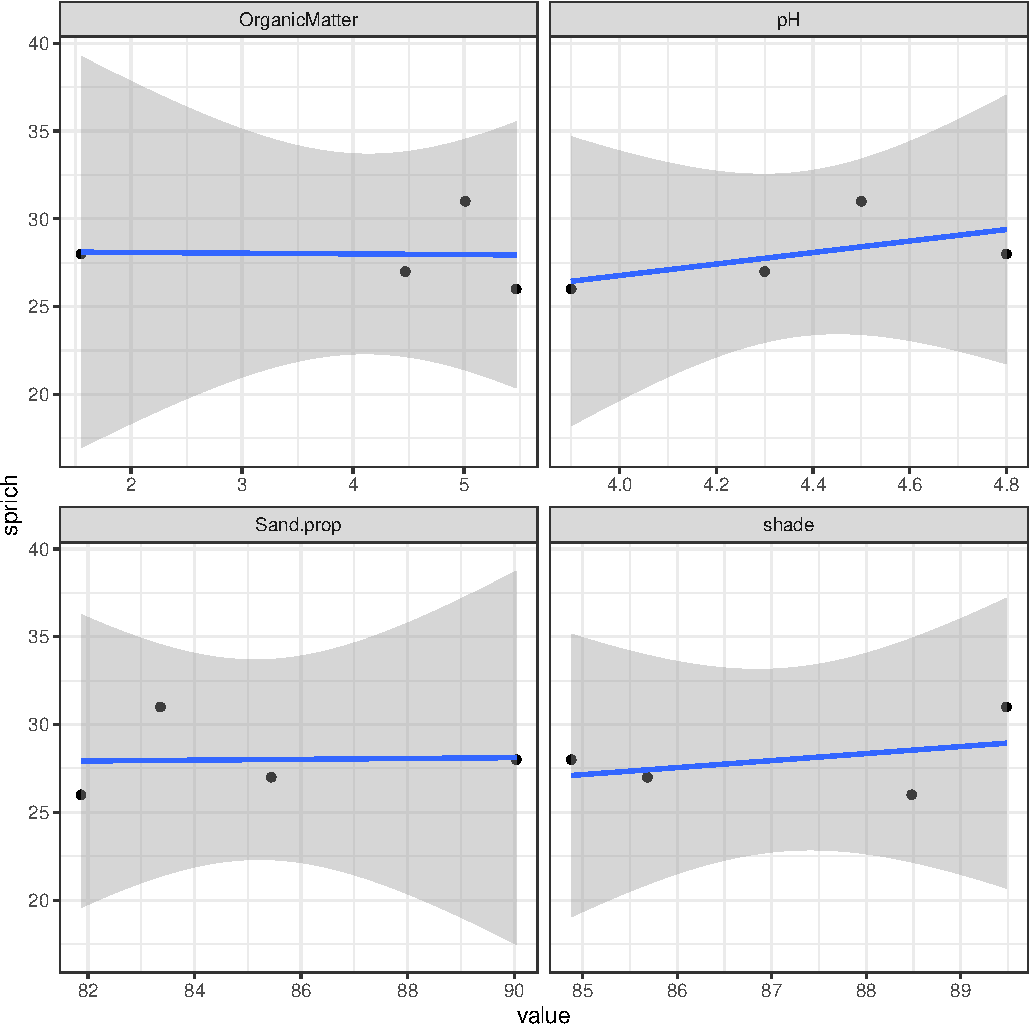
\includegraphics{ms_files/figure-latex/figName-1} 

}

\caption{\textbf{No - or \_ in the caption ref.} No space at the end of this line!}\label{fig:figName}
\end{figure}

Or if you already have the figure:

And cite it as Figure \ref{fig:fig2}.



\begin{figure}[H]

{\centering 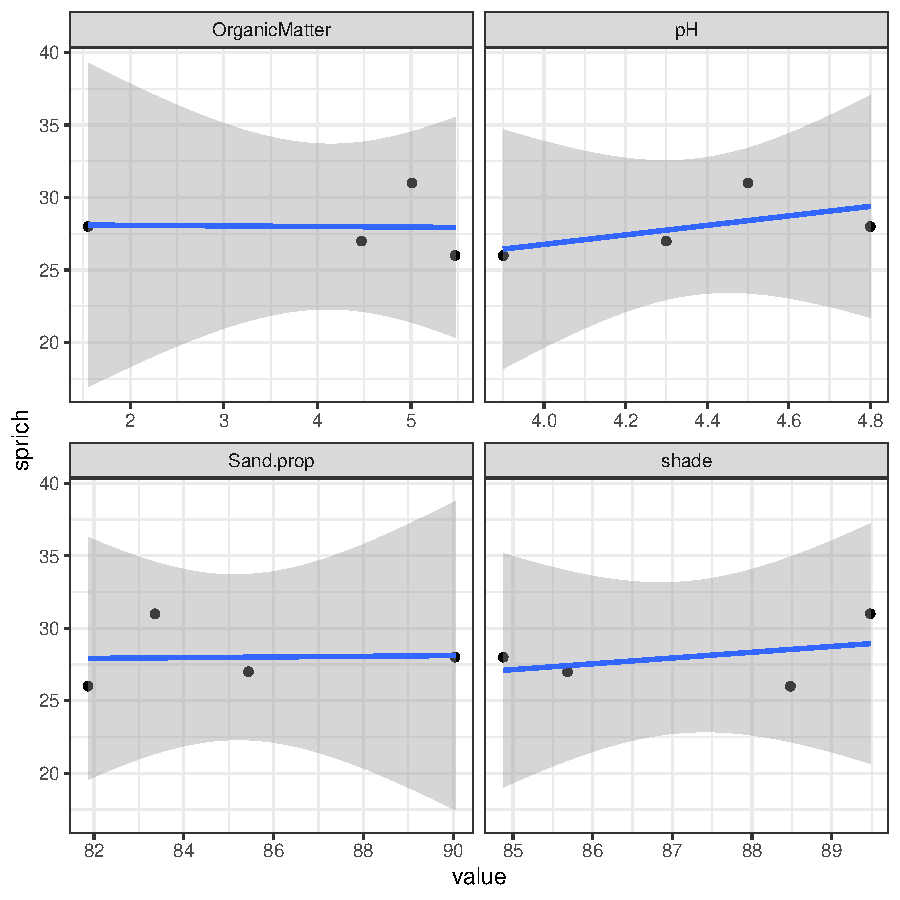
\includegraphics[width=0.7\linewidth,]{/Users/dli/github/workflow_demo/Figs/plot} 

}

\caption{\textbf{No - or \_ in the caption ref.} No space at the end of this line!}\label{fig:fig2}
\end{figure}

More details can be found at \href{https://bookdown.org/yihui/bookdown/}{here}.

\hypertarget{references}{%
\section{References}\label{references}}

\hypertarget{refs}{}
\begin{cslreferences}
\leavevmode\hypertarget{ref-adair_single-pool_2010}{}%
Adair, E. C., S. E. Hobbie, and R. K. Hobbie. 2010. Single-pool exponential decomposition models: Potential pitfalls in their use in ecological studies. Ecology 91:1225--1236.

\leavevmode\hypertarget{ref-clark_loss_2008}{}%
Clark, C. M., and D. Tilman. 2008. Loss of plant species after chronic low-level nitrogen deposition to prairie grasslands. Nature 451:712--715.

\leavevmode\hypertarget{ref-eriksson_seed_1993}{}%
Eriksson, O., and J. Ehrlén. 1993. Seed and microsite limitation of recruitment in plant populations. Oecologia 92:361--366.

\leavevmode\hypertarget{ref-williamson_dissolved_1999}{}%
Williamson, C. E., D. P. Morris, M. L. Pace, and O. G. Olson. 1999. Dissolved organic carbon and nutrients as regulators of lake ecosystems: Resurrection of a more integrated paradigm. Limnology and Oceanography 44:795--803.
\end{cslreferences}

\clearpage

\setcounter{page}{0}
\pagenumbering{arabic}
\setcounter{page}{1}

\setcounter{figure}{0}
\setcounter{table}{0}
\renewcommand {\thetable}{S\arabic{table}}
\renewcommand {\thefigure}{S\arabic{figure}}

\hypertarget{supporting-information}{%
\section{Supporting Information}\label{supporting-information}}

\hypertarget{figures-1}{%
\subsection{Figures}\label{figures-1}}



\begin{figure}[H]

{\centering 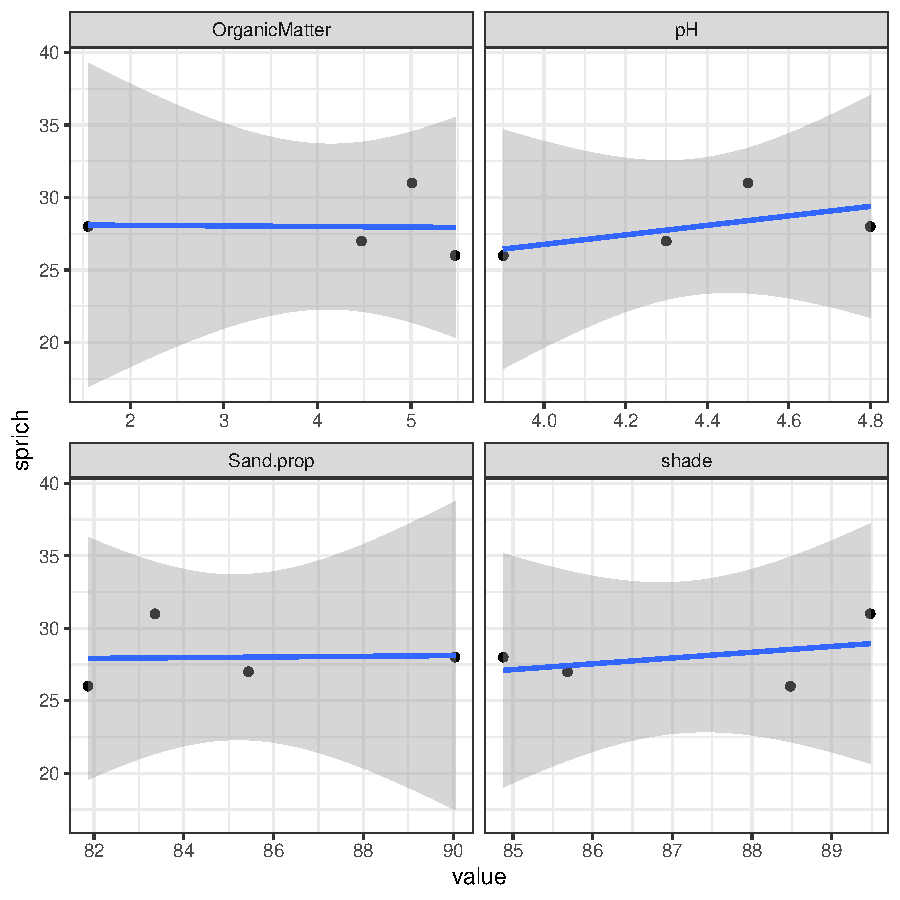
\includegraphics[width=0.7\linewidth,]{/Users/dli/github/workflow_demo/Figs/plot} 

}

\caption{\textbf{No - or \_ in the caption ref.} No space at the end of this line!}\label{fig:figS1}
\end{figure}

\end{document}
